\chapter{Qualitative Analysis of Doctors’ Perspectives on Telemedicine in Uzbekistan}

\section{Introduction}

This chapter presents a qualitative analysis of physicians’ perspectives on telemedicine in Uzbekistan. The aim is to identify practical challenges in current healthcare delivery and to derive functional and technical requirements for a telemedicine platform. The analysis builds on the research objectives outlined in Chapters 1.1--1.3 and addresses the following research question: How do doctors in Uzbekistan perceive, use, and evaluate telemedicine in routine practice, and what actionable requirements for a telemedicine platform can be derived from their experiences?

\section{Methodology}

The empirical basis of this study consists of fifteen semi-structured interviews conducted with physicians from Uzbekistan. The participants were selected using purposive sampling to ensure diversity in both geographic distribution and medical specialization. The sample includes physicians from regions such as Tashkent, Samarkand, Bukhara, Khorezm, Karakalpakstan (Nukus), Jizzakh, Kashkadarya, Surkhandarya, and Navoi, as well as from different specialties including general practice, cardiology, obstetrics and gynecology, pediatrics, and surgery. Participants were recruited through professional networks and direct outreach via email and messaging platforms. The selection aimed to capture a broad range of experiences with telemedicine across urban, semi-urban, and rural healthcare settings.

Each interview followed a structured guide consisting of seven thematic blocks: General Use and Attitudes, Video Calls, Appointment Scheduling, Data Collection and Management, Communication via Applications, Recording and Summarization, and Legal and Data Protection Aspects. Table~\ref{tab:mayring-survey-questions} summarizes the interview questions by category and descriptive label.

The analysis was conducted using qualitative content analysis following the approach proposed by Mayring (Mayring P., 2015). This method combines deductive and inductive category development in a systematic and transparent manner. In the first step, deductive main categories were defined based on the interview guide. Subsequently, inductive subcategories were developed through iterative analysis of the interview material. This involved paraphrasing, summarizing, and generalizing relevant text passages. The coding unit was defined as a sentence or a meaningful clause, while the context unit corresponded to the thematic interview blocks. All text segments were systematically assigned to categories based on predefined coding rules; multiple coding was permitted where statements addressed more than one thematic dimension.

During the analysis, categories were continuously refined to improve clarity and reduce overlap. Inclusion and exclusion criteria were defined for each category and supported by representative anchor quotes. The results were synthesized descriptively and analytically, including frequency-based observations where appropriate. A complete codebook, including category definitions and anchor examples, is provided in Appendix A. The full interview transcripts were translated into English and are documented separately in anonymized form.

\subsection{Complementary incorporation of patient perspectives}

The primary derivation of system requirements in this thesis is intentionally physician-centered. This choice follows from the role of physicians as workflow owners and clinical decision-makers in day-to-day care delivery, especially for appointment logic, documentation responsibilities, and risk-sensitive communication processes. Consequently, the requirement synthesis presented in Chapter~5 is anchored first in doctor interviews and subsequently reconciled with the implemented system architecture.

At the same time, patient perspectives were incorporated through two complementary channels. First, an exploratory assessment addressed access-related barriers and everyday digital habits relevant to telemedicine use. In methodological terms, this input is treated as problem-space evidence that supports triangulation and helps prioritize physician-derived requirements in relation to practical adoption constraints. It is not used for statistical generalization, nor as an independent basis for defining the core requirement set.

Second, patient perspectives are being integrated through ongoing prototype evaluation that focuses on usability, trust, and perceived impact during interaction with the developed applications. This evaluation is positioned as design- and acceptability-oriented evidence and is reported in the chapters that discuss implementation and user-interface realization. The following results section therefore concentrates on the physician interview corpus as the principal analytical source for the qualitative findings in this chapter.

\begin{longtable}{@{}l>{\RaggedRight\arraybackslash}p{0.62\textwidth}>{\RaggedRight\arraybackslash}p{0.20\textwidth}@{}}
\caption{Survey Questions by Category and Descriptive Label}\label{tab:mayring-survey-questions}\\
\toprule
Category & Question & Descriptive label \\
\midrule
\endfirsthead
\toprule
Category & Question & Descriptive label \\
\midrule
\endhead
\midrule
\multicolumn{3}{r@{}}{Continued on next page}\\
\endfoot
\bottomrule
\endlastfoot
A & Which telemedicine functions do you currently use in your practice? & Current telemedicine use \\
A & How has your daily work changed through telemedicine? & Impact on daily workflow \\
A & What expectations did you have of telemedicine before using it? & Initial expectations \\
A & How has your attitude toward telemedicine developed over time? & Attitude development over time \\
B & How often do you conduct videocalls with patients? & Frequency of videocalls \\
B & For what purposes do you mainly use videocalls? & Purpose of videocalls \\
B & What advantages do you see in using videocalls? & Perceived advantages \\
B & What challenges or problems occur during videocalls? & Challenges and problems \\
B & Are there patient groups for whom videocalls are particularly suitable or unsuitable? & Suitability by patient group \\
B & How do you assess the quality of medical care via videocall? & Quality of care via videocall \\
C & Do you use digital tools for appointment scheduling? If yes, which ones? & Use of digital appointment tools \\
C & How do you assess the acceptance of digital appointment scheduling among your patients? & Patient acceptance \\
C & What advantages and disadvantages do you see in digital appointment scheduling? & Pros and cons of digital scheduling \\
C & Were there technical or organizational problems when introducing digital appointment scheduling? & Implementation problems \\
D & How do you collect and store patient data digitally? & Digital data collection methods \\
D & Which systems or apps do you use for data exchange? & Systems for data exchange \\
D & How do you assess the security and reliability of these systems? & Data security and reliability \\
D & What advantages and risks do you see in digital data exchange and storage? & Advantages and risks of digital data \\
D & Have you ever experienced problems with data loss or data security? & Experience with data issues \\
D & How do you handle documentation and archiving of digital data? & Data documentation and archiving \\
E & Do you communicate with patients through special apps? If yes, how? & App communication with patients \\
E & Do you communicate with other doctors via digital platforms or apps? & App communication with colleagues \\
E & Which functions are most important to you in app communication (e.g., security, speed, documentation)? & Important app features \\
E & What challenges exist in digital communication with patients and colleagues? & Challenges in app communication \\
F & Do you use functions for automatic recording or summarization of videocalls? & Use of recording \\
F & How useful would such recording functions be for your work? & Usefulness of recording tools \\
F & Do you have improvement suggestions regarding recording and documentation? & Suggestions for improvement \\
G & How do you assess data protection and legal frameworks when using telemedicine functions? & Perception of data protection \\
G & Are there legal uncertainties that limit your telemedicine work? & Legal uncertainties \\
G & What kind of support do you wish regarding data protection and legal issues? & Desired legal support \\
\end{longtable}

\section{Results}

The findings indicate that telemedicine in Uzbekistan is currently practiced primarily through informal and fragmented digital communication channels. Rather than relying on integrated platforms, most physicians use common messaging applications such as Telegram or standard phone calls to communicate with patients. These interactions typically involve follow-up consultations, sharing of medical images or test results, and providing general medical advice. This pattern is consistent with broader telemedicine literature showing that practical adoption often precedes institutional integration (Bashshur et al., 2014; Shigekawa et al., 2018).

Video consultations are used as a supplementary tool rather than a primary mode of care delivery. Across the interview sample, weekly-or-more use is reported by roughly one-third of participants, monthly use by more than half, and rare or no use by a small minority. Across specialties, video consultations are perceived as useful for follow-up care, triage, and patient reassurance; however, they are generally not considered sufficient for diagnostic purposes because physical examination is not possible. This distribution is summarized in Figure~\ref{fig:mayring-video-call-frequency}.

\begin{figure}[H]
\centering
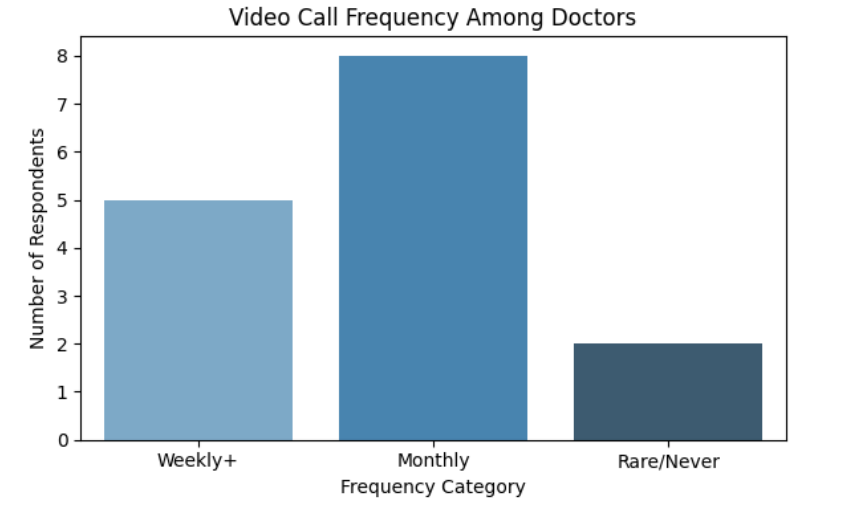
\includegraphics[width=\linewidth]{mayring_figure1.png}
\caption{Video Call Frequency}
\label{fig:mayring-video-call-frequency}
\end{figure}

Appointment scheduling remains largely manual. Most physicians rely on paper-based systems or telephone coordination, while only a small minority report using official digital scheduling systems and isolated ad hoc tools. In some urban settings, partial digital solutions such as electronic health record systems or pilot platforms exist, but these are not integrated into broader workflows. As a result, inefficiencies such as double-booking and redundant administrative work frequently occur. Figure~\ref{fig:mayring-scheduling-methods} illustrates this distribution of scheduling methods.

\begin{figure}[H]
\centering
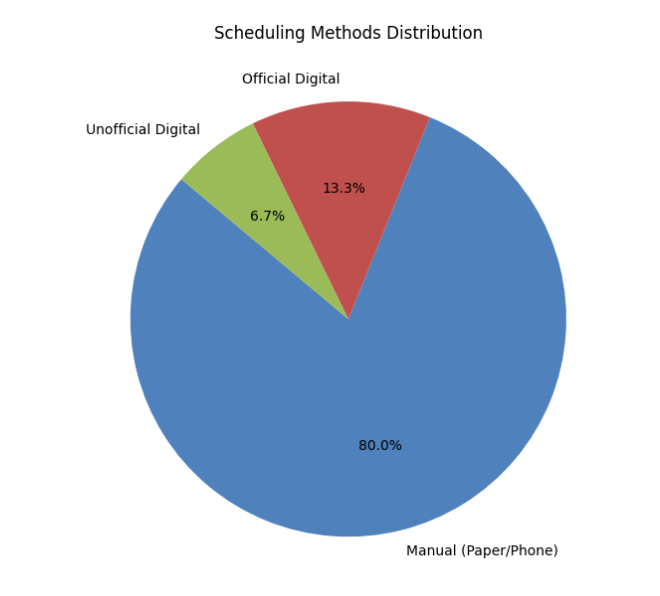
\includegraphics[width=\linewidth]{mayring_figure2.png}
\caption{Scheduling Methods Distribution}
\label{fig:mayring-scheduling-methods}
\end{figure}

Data management practices are characterized by a predominance of paper-based documentation combined with ad hoc digital storage solutions. Physicians often store patient data on personal devices, USB drives, or simple spreadsheet applications. This fragmented approach leads to significant operational risks, including frequent reports of data loss due to device failures, malware, or the absence of systematic backup procedures. Concerns regarding data security and legal uncertainty are widespread. Messaging applications are perceived as convenient, yet they are also recognized as insecure and not compliant with formal data protection standards. Many physicians further express uncertainty regarding legal responsibilities, particularly in relation to remote diagnosis, electronic prescriptions, and patient consent, which contributes to cautious behavior in remote settings. The reported prevalence of data-loss incidents is high, and legal uncertainty is nearly universal across the interview sample, as summarized in Figure~\ref{fig:mayring-data-loss-legal}.

\begin{figure}[H]
\centering
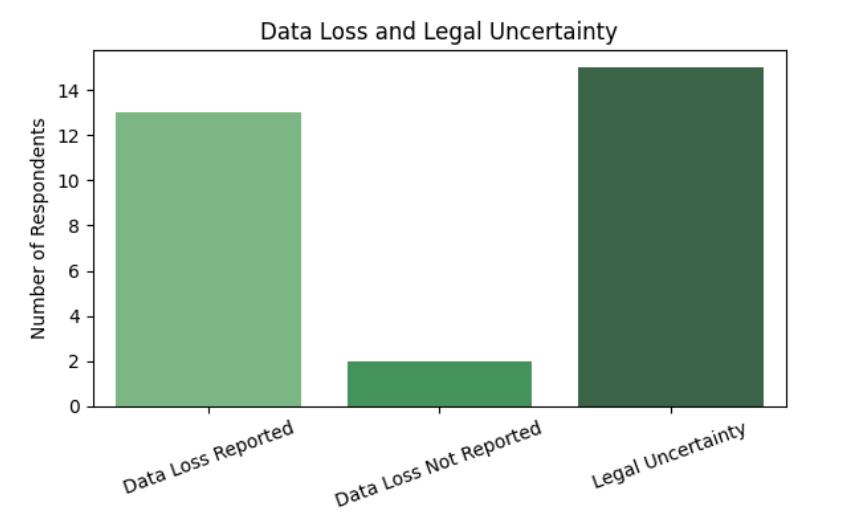
\includegraphics[width=\linewidth]{mayring_figure3.png}
\caption{Data Loss and Legal Uncertainty}
\label{fig:mayring-data-loss-legal}
\end{figure}

Another important finding relates to the impact of digital communication on work--life boundaries. Physicians report that asynchronous messaging creates expectations of constant availability, leading to increased workload outside regular working hours. This highlights the need for structured communication tools that allow better control over availability and response times. Despite these challenges, there is a clear demand for a centralized and secure telemedicine platform. Many participants emphasize the need for a government-approved solution that integrates communication, scheduling, and data management functionalities while ensuring compliance with legal and data protection requirements.

Differences between medical specialties and regional contexts are also evident. For example, cardiology shows a comparatively higher adoption of telemedicine for chronic disease management and exchange of diagnostic data, whereas surgical disciplines remain more skeptical due to the hands-on nature of their work. Urban healthcare providers tend to adopt digital tools more readily, while semi-rural and rural settings remain strongly dependent on paper-based processes.

\section{Discussion}

The findings demonstrate that telemedicine in Uzbekistan is already present in everyday clinical practice, albeit in an informal and unstructured manner. The widespread use of consumer messaging applications indicates both a strong demand for digital healthcare solutions and a lack of adequate institutional infrastructure. These observations are consistent with the broader health system challenges outlined in Chapter 1. While digital health has been identified as a strategic priority, its implementation remains uneven and constrained by infrastructural, organizational, and regulatory limitations.

From a system design perspective, the results imply several key requirements for a telemedicine platform. These include secure and compliant communication channels, integrated appointment scheduling, reliable data storage solutions, and clear mechanisms for managing legal and ethical responsibilities. In addition, user-centered features that address workload management and heterogeneous levels of digital literacy appear necessary to support adoption across diverse practice settings, in line with established adoption and implementation frameworks (Venkatesh et al., 2003; Greenhalgh et al., 2017).

\section{Conclusion}

This analysis shows that physicians in Uzbekistan are already engaging in telemedicine practices through informal digital tools, particularly for follow-up care and patient communication. However, the lack of integrated systems, combined with data security risks and legal uncertainty, limits the effectiveness and scalability of these practices. While the sample of fifteen interviews provides valuable insights across different regions and specialties, it is not statistically representative. The findings are therefore most applicable to similar healthcare contexts characterized by limited digital infrastructure and transitional regulatory environments. To enhance reliability in future work, additional validation procedures such as inter-coder agreement or participant feedback could be incorporated. Nevertheless, the results provide an empirical foundation for the development of a structured and context-appropriate telemedicine platform.

